\chapter{Original Honours Proposal}
\subfile{../proposal/proposal}


\chapter{Ideal System Architecture}
\label{chap:architecture}
Beyond specific sensor design and occupancy detection algorithms, a core goal of this project is to create a system that is designed to operate as a useful Thing in a real-world \iot environment, as the key advantage of Things is the ``disruptive level of innovation''\cite{atzori2010internet} brought about by their ability to be combined in ways unforeseen (yet still enabled) by their creators. This architecture involves careful consideration of the embedded hardware that will drive the system, as well as the communications protocols utilised between the sensor and devices interested in the sensor's information.

\section{Protocols}
\label{sec:litreview:architecture:protocols}
% From; https://openwsn.atlassian.net/wiki/pages/viewpage.action?pageId=29196353
\begin{table}
\centering
\begin{tabular}{|c|c|}
\hline
\multicolumn{2}{|c|}{\acs{rest}} \\ \hline
\textbf{Application} & \acs{coap} \\ \hline
\textbf{Transport} & UDP \\ \hline
\textbf{IP / Routing} & IETF \acs{roll} \\ \hline
\textbf{Adaptation} & IETF \acs{lowpan} \\ \hline
\textbf{Medium Access} & IEEE \lmed \\ \hline
\textbf{Physical} & IEEE \lphy \\ \hline
\end{tabular}
\caption{Proposed protocol stack}
\label{tab:litreview:protostack}
\end{table}

In an ideal smart-home environment, the sensor systems used will communicate with each other wirelessly. As the complete sensor system has low power requirements to enable battery operation, it is important to prioritise those protocols and architectures that minimise power usage while still enabling the necessary wireless communication. The system will also ideally exist in a system with other identical sensors (one for each room in a residence), thus it is important to prioritise those protocols which allow multiple identical sensor systems to coexist on the same network without conflict, and to be uniquely addressable and identifiable. In recent years, many developments have been made in the \iot arena, with standards emerging specifically designed for low-power embedded devices to communicate between themselves and bigger systems that address these and other unique needs, across the entire protocol stack. 

Palattella \etal \cite{palattella2013standardized} propose a protocol stack that aligns with the above requirements, with the key advantage being a wholly standardized implementation of the stack exists. This implementation is based on TCP/IP, uses the latest IEEE and IETF \iot standards, and is free from proprietary protocol restrictions (unlike ZigBee 1.0 devices, for instance). \Fref{tab:litreview:protostack} shows the full stack proposed. The key components of this proposal are the introduction of \acs{coap} at the application layer, \acs{roll} at the IP / Routing layer and \acs{lowpan} at the Adaptation layer.

Above the application layer, Guinard \etal \cite{guinard2012search} propose the use of \rest over \ws as a method of exchanging information between sensor systems. Their data suggests that \rest is easier to use than \ws, and the key advantage of a \ws based approach is its ability to represent much more complex data and abstractions, which are unnecessary in this project's situation.

\coap \cite{kovatsch2013coap} is an application layer protocol designed to replace HTTP as a way of transmitting RESTful information between clients. The chief advantage of \coap over HTTP is it compresses the broad-strokes of the HTTP feature set into a binary language that is much more suitable for transmission over low-bandwidth and low-power links, such as those discussed here.

\roll \cite{rfc6550} is a routing protocol designed for low power environments, allowing low power nodes to create and maintain a mesh network between themselves, allowing, among other things, the routing of packets to a ``root'' node and back again. \roll is particularly suited to the routing situation of our proposed architecture, as individual sensors do not need to communicate with one another, but rather report back to a larger node (further discussed in \Fref{subsec:litreview:architecture:devices}).

\lowpan \cite{shelby20116lowpan} is a compression and formatting specification to allow IPv6 packets to be sent over an \lwifi based network. Optimisations are found in the reduction of the size of \lowpan packets, IPv6 addresses as well as redesigning core Internet Protocol algorithms so that they can run with low power consumption on participating devices.

\section{Devices}
\label{subsec:litreview:architecture:devices}
\begin{figure}
\centering
\begin{tikzpicture}[node distance=1.7cm]
\node (interwebs) [cbox] {Internet};
\node (http) [dashbox, left=of interwebs] {\small HTTP};
\node (rpi) [box, below=of http] {Smart Gateway / Processor};
\node (coap) [dashbox, right=of rpi] {\small \acs{coap}};
\node (mesh) [cbox, right=of coap] {WPAN};
\node (embed1) [box, below left=of mesh] {Sensor};
\node (embed2) [box, below right=of mesh] {Sensor};

\draw [line] (interwebs) -- (http);
\draw [line] (http) -- (rpi);
\draw [line] (rpi) -- (coap);
\draw [line] (coap) -- (mesh);
\draw [line] (mesh) -- (embed1);
\draw [line] (mesh) -- (embed2);
\end{tikzpicture}
\caption{Proposed system architecture}
\label{fig:litreview:devices}
\end{figure}

In addition to the protocol stack used, how these nodes relate to each other is also an important consideration. Part of what will inform these decisions are the requisite processing power and internet connectivity required to successfully execute all elements of the sensing system. Kovatsch \cite{kovatsch2013coap} provides a constructive classification system to consider this, by describing three classes of resource constrained devices that would benefit from \coap, and each can provide different levels of security for an IP stack;

\begin{itemize}
 \item \emph{Class 0}: ``not capable of running an RFC-compliant IP stack in a secure manner. They require application-level gateways to connect to the Internet.''
 \item \emph{Class 1}: Able to connect to the internet with some ``integrated security mechanisms''. Are unable to employ full HTTP with TLS.
 \item \emph{Class 2}: Normal Internet nodes, able to use the full HTTP stack with TLS.
\end{itemize}

The devices that we propose the sensors will connect to are the likes of the Arduino, which can be classified as class 0 or possibly class 1 devices. Due to their insecurity and difficulty running a fully fledged IP stack, Guinard \etal \cite{guinard2011internet} propose the use of a ``Smart Gateway'' system to bridge the wider internet and these sensor systems. This gateway would be able to communicate with the sensor systems over \coap and \lwifi, as well as receive API requests via HTTP from a traditional TCP/IP network to forward on to these sensors.

The Thermosense paper \cite{beltran2013thermosense} proposes several different algorithms to process the raw sensing data into the occupancy estimates (further discussed in \Fref{sec:litreview:thermalsensors}), all of which are fairly computationally expensive. Because of this, it would be non-trivial to implement these algorithms on the embedded sensing devices themselves. This problem is already resolved in our proposed system, as the aforementioned ``Smart Gateway'' can easily also take on the task of processing the raw sensor data into estimates which it can relay to interested parties over its HTTP-based API. A visualisation of this proposed system is shown in \Fref{fig:litreview:devices}.

\begin{landscape}
\chapter{Code Listings}


\section{ThingLib}
\subsection{cam.py}
\inputminted[fontsize=\footnotesize,breaklines=true,numbers=right]{python}{../../code/processing/thinglib/cam.py}
\subsection{pxdisplay.py}
\inputminted[fontsize=\footnotesize,breaklines=true,numbers=right]{python}{../../code/processing/thinglib/pxdisplay.py}
\subsection{features.py}
\inputminted[fontsize=\footnotesize,breaklines=true,numbers=right]{python}{../../code/processing/thinglib/features.py}

\section{Arduino Sketch}
\inputminted[fontsize=\footnotesize,breaklines=true,numbers=right]{C++}{../../code/mlx90620_driver/mlx90620_driver.ino}

\end{landscape}


\chapter{Full Results}


\section{Classifier Experiment Set 1}
\label{sec:results:cexp1}
\subsection{combined-exp-all-export}
\inputminted[fontsize=\footnotesize,breaklines=true]{text}{../data/processed/classification-expset-1/combined-exp-all-export.txt}
\clearpage

\subsection{combined-exp-all-noresample-export}
\inputminted[fontsize=\footnotesize,breaklines=true]{text}{../data/processed/classification-expset-1/combined-exp-all-noresample-export.txt}
\clearpage

\subsection{combined-exp-excl0-export}
\inputminted[fontsize=\footnotesize,breaklines=true]{text}{../data/processed/classification-expset-1/combined-exp-excl0-export.txt}
\clearpage

\subsection{combined-exp-excl0-noresample-export}
\inputminted[fontsize=\footnotesize,breaklines=true]{text}{../data/processed/classification-expset-1/combined-exp-excl0-noresample-export.txt}
\clearpage

\subsection{combined-exp-excl0-linreg}
\inputminted[fontsize=\footnotesize,breaklines=true]{text}{../data/processed/classification-expset-1/combined-exp-excl0-linreg.txt}
\clearpage

\subsection{subexp1-all-export}
\inputminted[fontsize=\footnotesize,breaklines=true]{text}{../data/processed/classification-expset-1/subexp1-all-export.txt}
\clearpage

\subsection{subexp2-all-export}
\inputminted[fontsize=\footnotesize,breaklines=true]{text}{../data/processed/classification-expset-1/subexp2-all-export.txt}
\clearpage

\subsection{subexp3-all-export}
\inputminted[fontsize=\footnotesize,breaklines=true]{text}{../data/processed/classification-expset-1/subexp3-all-export.txt}
\clearpage

\subsection{subexp4-all-export}
\inputminted[fontsize=\footnotesize,breaklines=true]{text}{../data/processed/classification-expset-1/subexp4-all-export.txt}
\clearpage

\subsection{subexp5-all-export}
\inputminted[fontsize=\footnotesize,breaklines=true]{text}{../data/processed/classification-expset-1/subexp5-all-export.txt}
\clearpage

\subsection{subexp6-all-export}
\inputminted[fontsize=\footnotesize,breaklines=true]{text}{../data/processed/classification-expset-1/subexp6-all-export.txt}
\clearpage

\subsection{subexp7-all-export}
\inputminted[fontsize=\footnotesize,breaklines=true]{text}{../data/processed/classification-expset-1/subexp7-all-export.txt}
\clearpage

\subsection{subexp8-all-export}
\inputminted[fontsize=\footnotesize,breaklines=true]{text}{../data/processed/classification-expset-1/subexp8-all-export.txt}
\clearpage

\subsection{subexp9-all-export}
\inputminted[fontsize=\footnotesize,breaklines=true]{text}{../data/processed/classification-expset-1/subexp9-all-export.txt}
\clearpage


\chapter{Physical Form}
To enable the prototype to be easily mounted on the ceiling, the prototype was placed on a flat board with feet that would enable it to be screwed into a pole, and the pole extended to jam the sensor against the ceiling and the floor using the pole (\Fref{fig:pictures:protob1}, \Fref{fig:pictures:protoact}). Due to a wireless module and battery pack being added to the Raspberry Pi, it was feasible for the sensor to operate entirely wirelessly for several hours. However, in most cases it was more convenient to operate using wired power and Ethernet.

\begin{figure}[H]
\centering
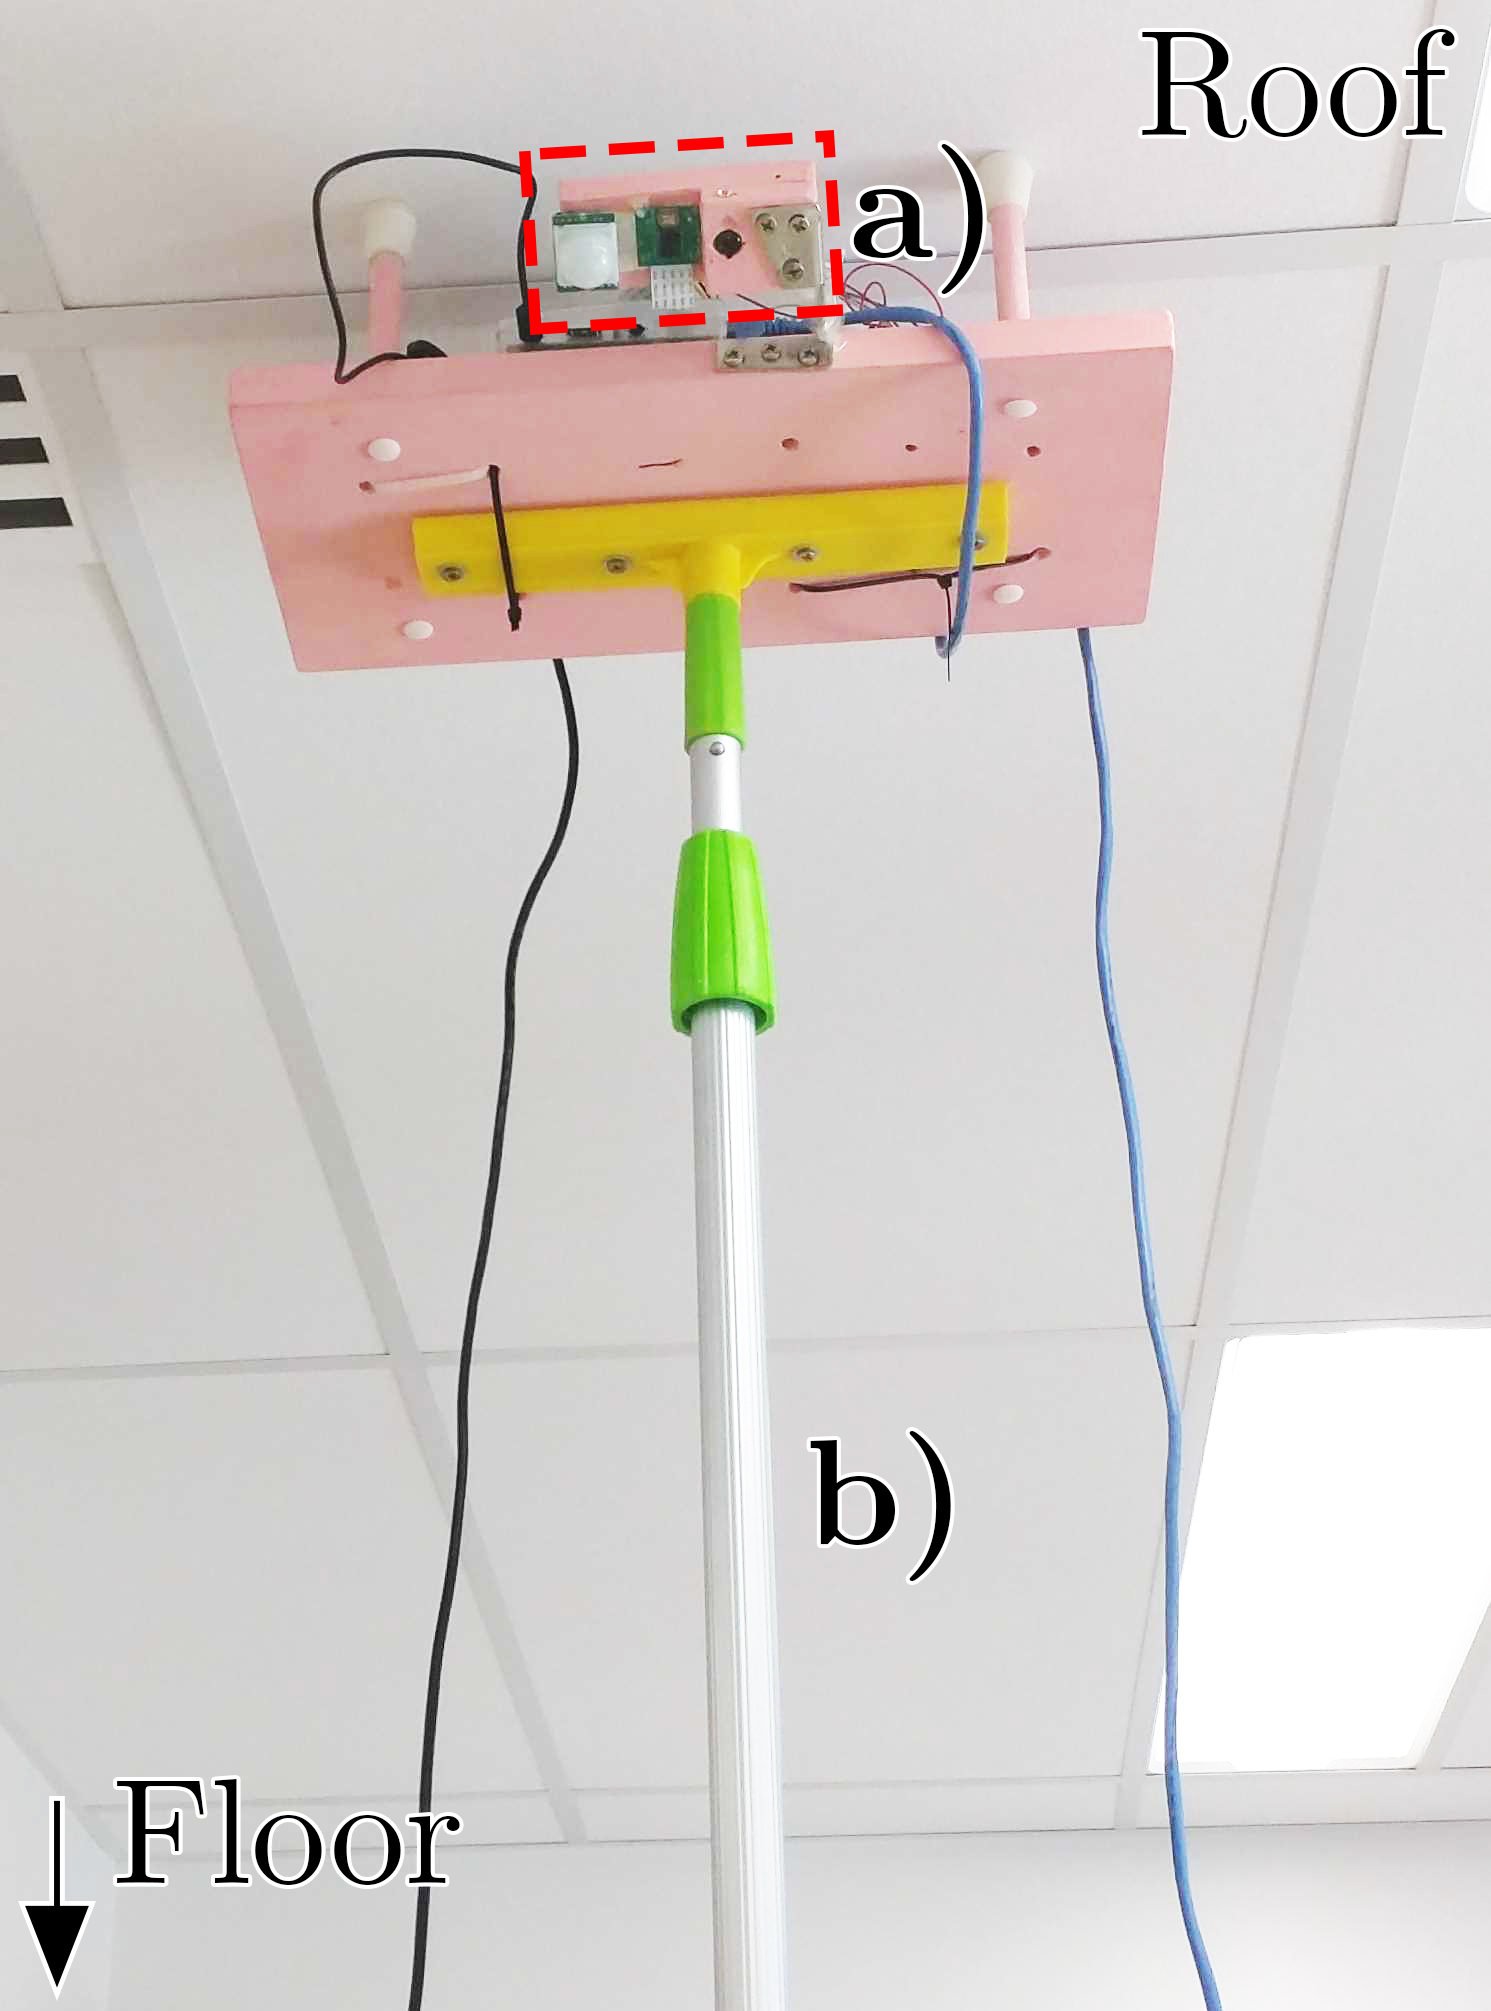
\includegraphics[height=0.5\textheight]{../diagrams/prototype-mounted-ceiling.jpg}
\caption{Prototype in action}
\label{fig:pictures:protoact}
\end{figure}

\begin{figure}[H]
\centering
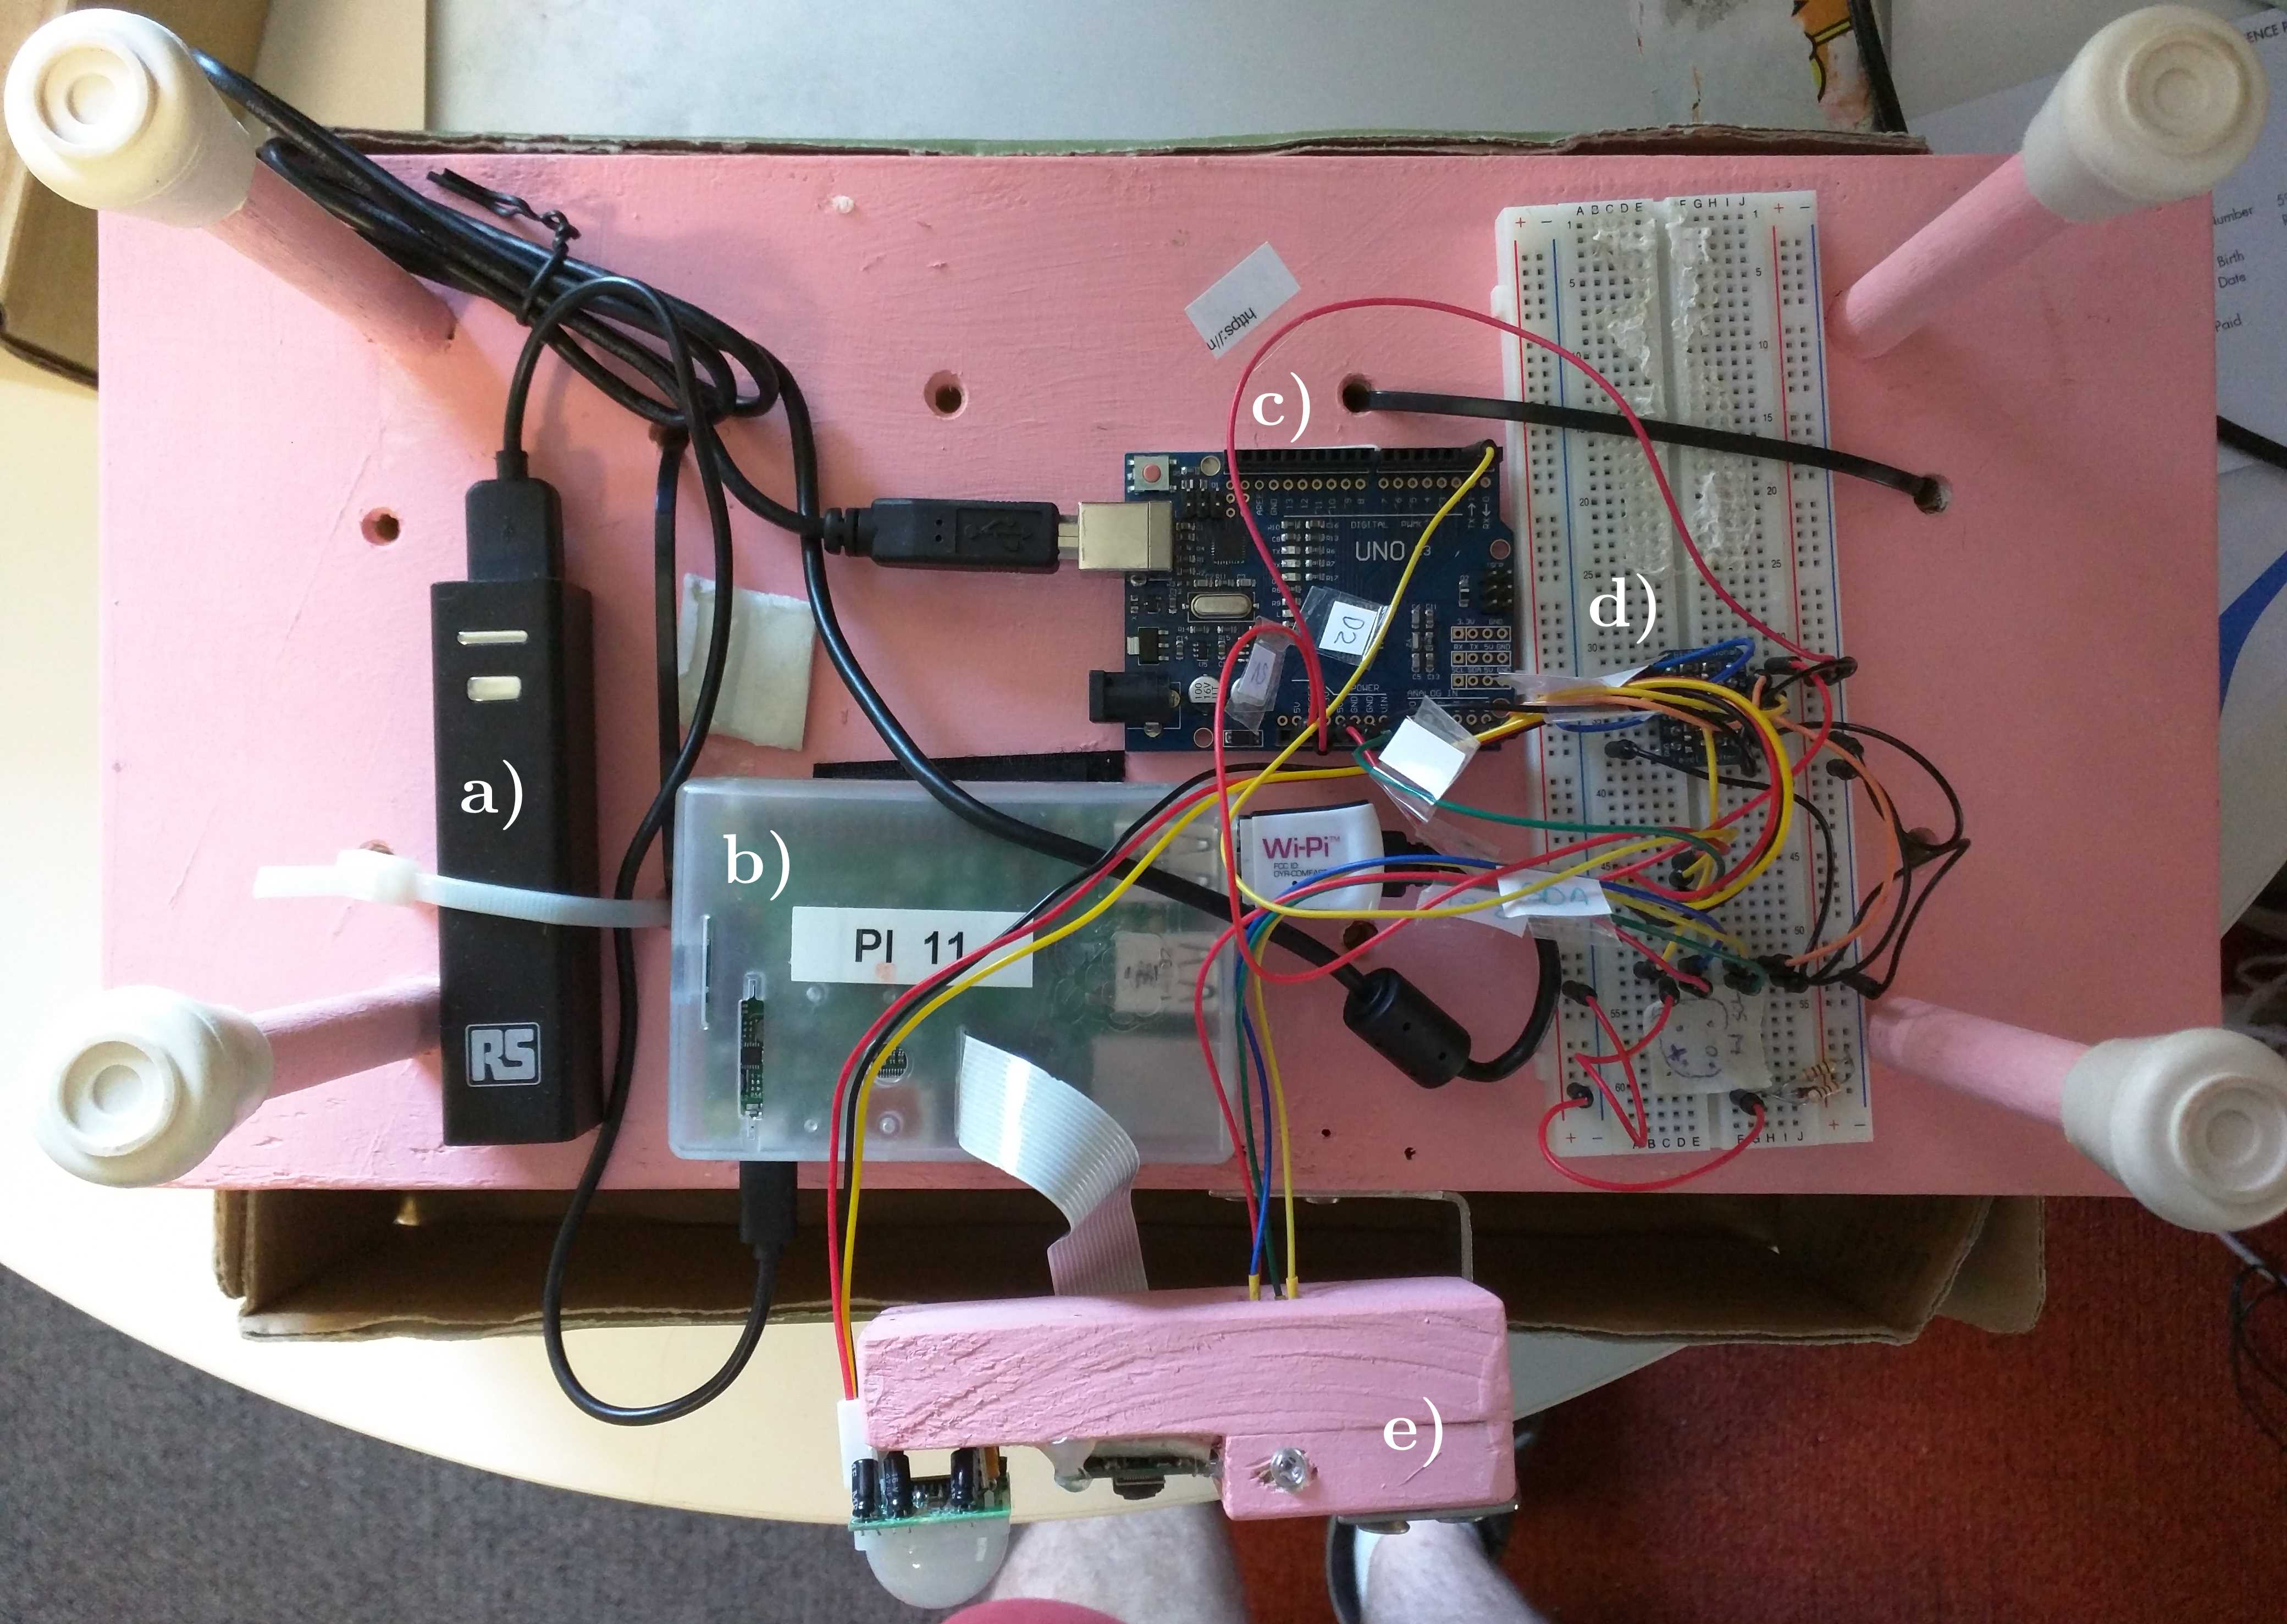
\includegraphics[width=\textwidth]{../diagrams/prototypeb-1.jpg}
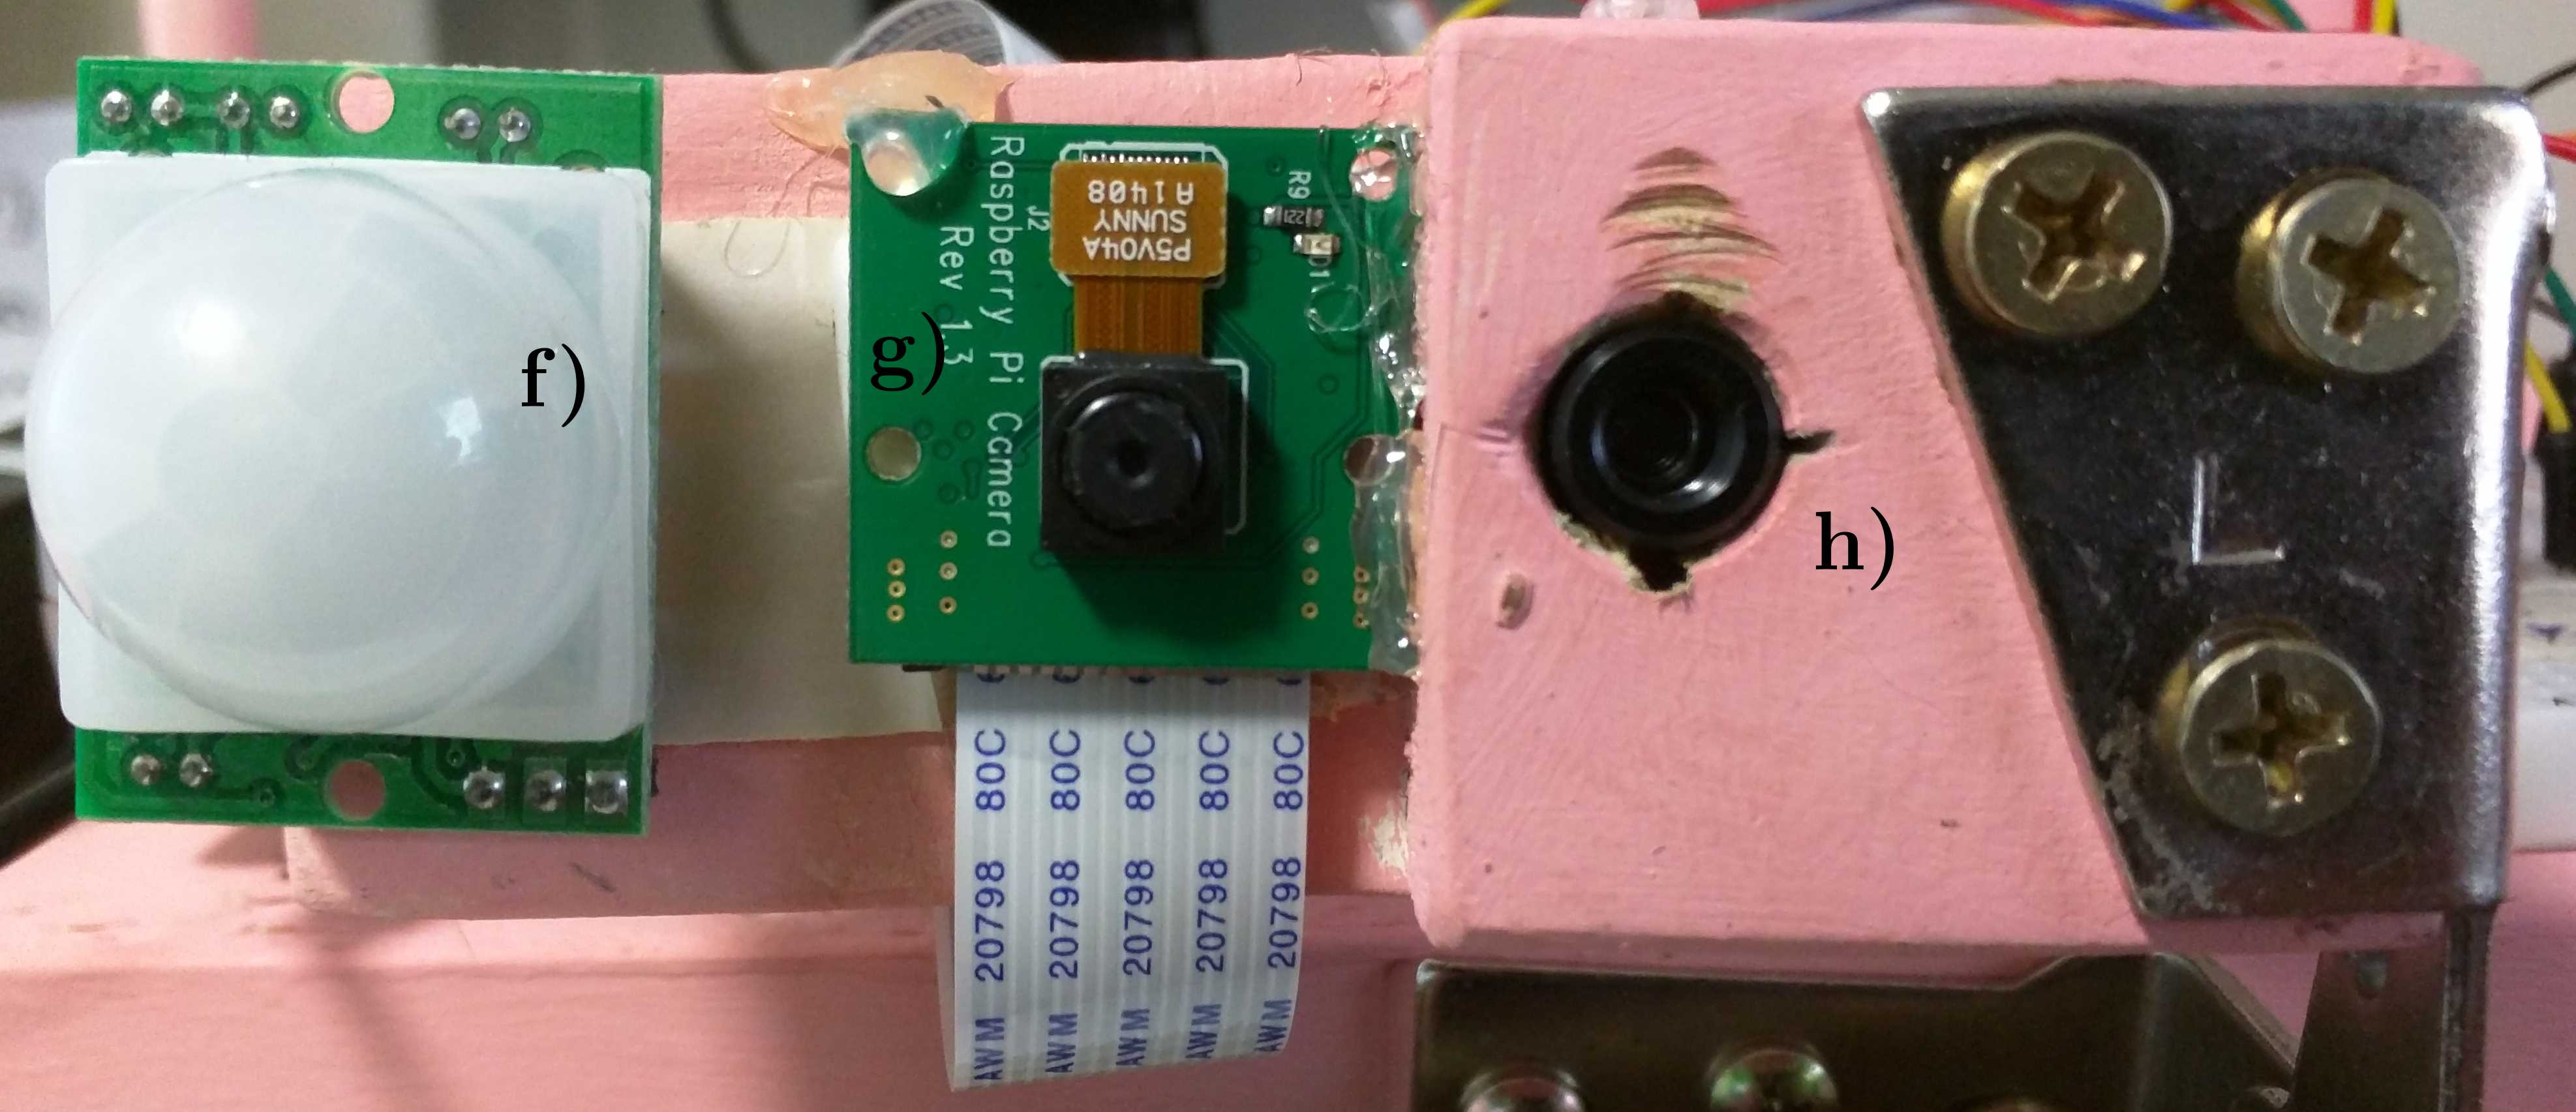
\includegraphics[width=\textwidth]{../diagrams/prototypeb-2.jpg}
{\small
\begin{multicols}{2}
\begin{enumerate}[a)]
 \item Battery pack
 \item Raspberry Pi
 \item Arduino
 \item Level-shifting circuitry
 \item Movable sensor mount
 \item PIR
 \item Camera
 \item \mlx
\end{enumerate}
\end{multicols}
}
\caption{Prototype Physical Form}
\label{fig:pictures:protob1}
\end{figure}